\documentclass[a4paper,12pt]{article}
\usepackage{graphicx} % Required for inserting images
\usepackage[utf8]{inputenc}
\usepackage{subcaption}
\usepackage{caption}
\usepackage{amsmath}
\usepackage[spanish,es-tabla]{babel}
\usepackage[useregional]{datetime2}
\usepackage{multicol}
\usepackage{float}
\usepackage{geometry}
\usepackage{url}
\usepackage[backend=biber,sorting=none]{biblatex}

\usepackage{siunitx}
\usepackage{booktabs}
\usepackage{array}
\usepackage{geometry}
\usepackage{graphicx}
\usepackage{float}
\usepackage{hyperref}
\usepackage{xcolor}
\usepackage{multirow}
\usepackage{amsmath}
\usepackage{amssymb}
\usepackage{enumitem}
\bibliography{rsc/ref}

% Configuración de márgenes
\geometry{
    left=2cm,    % Margen izquierdo
    right=2cm,   % Margen derecho
    top=3cm,     % Margen superior
    bottom=3cm   % Margen inferior
}


\begin{document}
    \begin{titlepage}
    \centering
    
    \begin{minipage}{0.2 \textwidth}
        \centering
        
\includegraphics[width=0.5 \textwidth]{rsc/format/uaq.png}
    \end{minipage}
    \hfill
    \begin{minipage}{0.4\textwidth}
        \centering
        {Universidad Autónoma de Queretaro \par}
        \vspace{0.2cm}
        {Facultad De Ingeniaría\par}
    \end{minipage}
    \hfill
    \begin{minipage}{0.3 \textwidth}
        \centering
        
\includegraphics[width=1 \textwidth]{rsc/format/fi.png}
    \end{minipage}
    
    \vspace{2cm}
    
    {\LARGE \bfseries Algoritmo Genetico Dicotomico \par}
    
    \vspace{1.5cm}
    
        {\Large \bfseries Algoritmos Metaheuristicos \\ Tarea 2\par}
    
    \vfill
    
    {\large P R E S E N T A} \par
    \vspace{0.5cm}
    {\Large \bfseries Ing. Daniel Eduardo González Alvarado\par}
    
    \vspace{2cm}
    
    {\large Profesor}\par
    \vspace{0.5cm}
    {\Large \bfseries Dr. Marco Antonio Aceves Fernández\par}
    
    \vfill
    
    \raggedleft {12 de Septiembre de 2025}
    
\end{titlepage}
    \pagenumbering{roman}
    \tableofcontents
    \clearpage % Asegura que el texto comience en una nueva página
    
    \newpage
    \pagenumbering{arabic}
    \section{Introducción}

Los algoritmos genéticos (AG) son una técnica de optimización inspirada en los principios de la evolución natural y la genética
basados en la mecánica de selección natural. Combinando la supervivencia del más apto con la reproducción sexual, con intercambio
de información estructurada~\cite{marcos2010introduccion}. 

En la naturaleza, los organismos más aptos tienen una mayor probabilidad de sobrevivir y reproducirse, transmitiendo sus genes
a la siguiente generación. De manera similar, en los AG, las soluciones potenciales (individuos) se representan como cadenas de
caracteres (cromosomas) y se evalúan mediante una función de aptitud que mide su calidad. De tal manera que la combinación de buenos
ancestros puede generar descendencia aún mejor.

Estos algoritmos se utilizan para resolver problemas complejos mediante
la simulación de procesos evolutivos, como la selección, el cruce y la mutación. Los AG son especialmente útiles en problemas donde el espacio de búsqueda es grande y no se dispone de
una solución analítica directa.

\subsection{Conceptos Básicos}
\begin{itemize}
    \item \textbf{Población:} Conjunto de soluciones candidatas que evolucionan a lo largo del tiempo.
    \item \textbf{Generación:} Cada iteración del algoritmo, donde se aplican los operadores genéticos.
    \item \textbf{Cromosoma:} Representación de una solución en la población, comúnmente como una cadena de bits.
    \item \textbf{Alelo:} Valor específico que puede tomar un gen en un cromosoma.
    \item \textbf{Gen:} Elemento básico de un cromosoma, que representa una característica de la solución.
\end{itemize}

\begin{figure} [H]
    \centering
    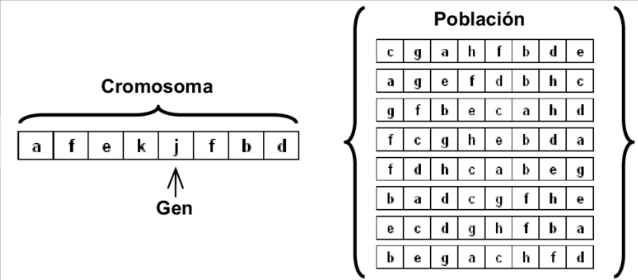
\includegraphics[width=0.5\textwidth]{C:/Users/death/Documents/Maestria/MCIA/Semestre_2/Metaheuristica/Reportes/Alg_Gen/rsc/img/genec.png}
    \caption{Representación de Poblacion y Cromosoma}\label{Poblacion}
\end{figure}

\subsection{Componentes de los Algoritmos Genéticos}
\begin{itemize}
    \item \textbf{Codificación de individuos:} Representación de las posibles soluciones del problema,
        comúnmente en forma de cadenas binarias, vectores o estructuras más complejas.
    
    \item \textbf{Función de aptitud (fitness):} Mide la calidad de cada individuo dentro de la población,
        es decir, qué tan buena es una solución respecto al objetivo del problema.
    
    \item \textbf{Población inicial:} Conjunto de individuos generados aleatoriamente o a partir de
        heurísticas, que servirán como punto de partida para la evolución.
    
    \item \textbf{Operadores genéticos:}
    \begin{itemize}
        \item \textbf{Selección:} Proceso mediante el cual se eligen los individuos que participarán en la reproducción, 
            favoreciendo a los de mayor aptitud.
            \begin{itemize}
                \item \textbf{Selección por torneo:} Se seleccionan aleatoriamente varios individuos y se elige el mejor entre ellos.
                \item \textbf{Selección por ruleta:} Cada individuo tiene una probabilidad de ser seleccionado proporcional a su aptitud.
                \item \textbf{Selección por rango:} Los individuos se ordenan según su aptitud y se asignan probabilidades de selección basadas en su posición en el ranking.
            \end{itemize}
        \item \textbf{Cruzamiento (crossover):} Combina el material genético de dos padres para generar descendencia con
            características de ambos.
            \begin{itemize}
                \item \textbf{Cruzamiento de un punto:} Se selecciona un punto de corte en los cromosomas de los padres y se intercambian las partes posteriores a ese punto.
                \item \textbf{Cruzamiento de k puntos:} Se seleccionan k puntos de corte y se intercambian las secciones entre esos puntos.
                \item \textbf{Cruzamiento aritmético:} Se combinan los valores de los padres mediante una operación aritmética (por ejemplo, promedio).
                \item \textbf{Cruzamiento de orden:} Utilizado en problemas de permutación, donde se preserva el orden relativo de los genes.
                \item \textbf{Cruzamiento de ciclo:} También para problemas de permutación, donde se identifican ciclos en los cromosomas de los padres para crear hijos.
                \item \textbf{Cruzamiento basado en la posición:} Se seleccionan posiciones específicas en los cromosomas de los padres para formar el hijo.
                \item \textbf{Cruzamiento de mezcla:} Se combinan segmentos de los padres de manera aleatoria.
            \end{itemize}
        \item \textbf{Mutación:} Introduce variaciones aleatorias en los individuos para mantener la diversidad genética y
            evitar la convergencia prematura.
    \end{itemize}
    
    \item \textbf{Criterios de paro:} Condiciones que determinan el final de la ejecución del algoritmo, como alcanzar un 
        número máximo de generaciones o una solución suficientemente buena.
\end{itemize}

\begin{figure}[H]
    \centering
    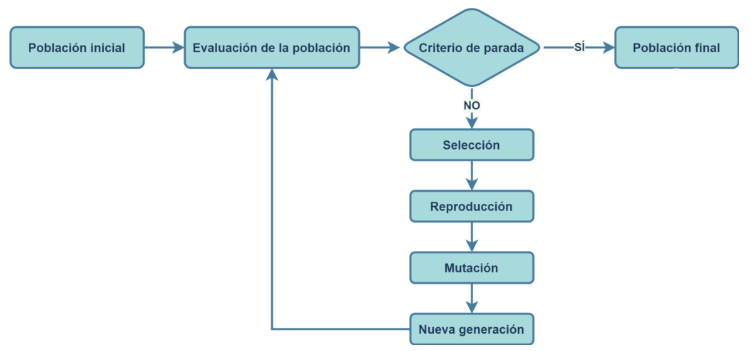
\includegraphics[width=0.8\textwidth]{C:/Users/death/Documents/Maestria/MCIA/Semestre_2/Metaheuristica/Reportes/Alg_Gen/rsc/img/Diagrama.png}
    \caption{Ciclo de un Algoritmo Genético}\label{diag}
\end{figure}

\subsection{Aplicacion a Algoritmo Dicotómico}

Para nuestro problema, desarrollaremos un AG que busque los mejores individuos según nuestra función de aptitud, la cual es $f(x) = x^2$.
Por lo tanto tomaremos en cuenta los siguientes aspectos:

\begin{itemize}
    \item Aptitud entre 0 y 1.
    \item Cromosoma: Binario de 6 bits.
    \item Alelos: 0 y 1.
    \item Función de aptitud: $f(x) = x^2$.
    \item Espacio de búsqueda: \{-1, 1\}[0, 63].
\end{itemize}

\begin{figure} [H]
    \centering
    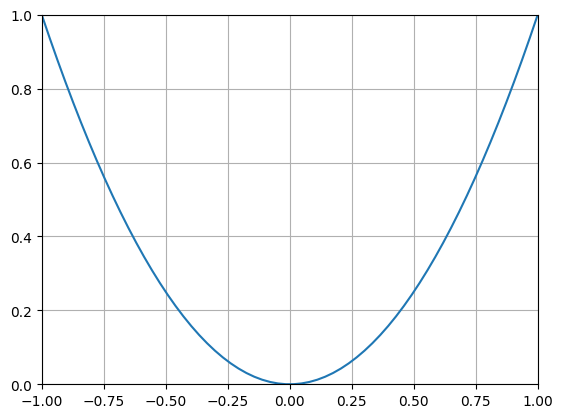
\includegraphics[width=0.5\textwidth]{C:/Users/death/Documents/Maestria/MCIA/Semestre_2/Metaheuristica/Reportes/Alg_Gen/rsc/img/funcion.png}
    \caption{Funcion de Aptitud $f(x) = x^2$}\label{funcion}
\end{figure}
    \section{Desarrollo}
% Metodologia / Desarrollo

    %\section{Resultados}
% Se muestran e interpretan los resultados como se obtuvieron


    \section{Discusión}
% Interpretacion propia de los datos

A lo largo del desarrollo del proyecto podemos ver que la implementacion correcta de cada etapa es primordial para el correcto funcionamiento
del AG esto toma especial relevancia al momento de mencionar que no se implemento la mutacion ya que este paso nos permitiria tener un mayor
grado de exploracion del espacio de soluciones, lo cual podria llevarnos a encontrar mejores soluciones en menos generaciones y de esta manera
evitar el estancamiento, ademas esto podria hacer que nuestro super individuo de la generacion 0 se mantenga siempre como el mejore.

Otro punto a destacar es como el cambio en el metodo de cruce afecta el rendimiento del algoritmo, en este caso el cruce por un punto
mostro ser mas efectivo que el cruce con dos puntos, esto puede deberse a que al tener un solo punto de corte se mantiene una mayor 
parte de la informacion genetica de los padres, lo que permite que las soluciones generadas sean mas cercanas a las mejores soluciones 
encontradas hasta el momento. Aunque por otro lado el usar dos puntos hace que la aptitud crezca mas rapidamente, pero esto puede llevar a que
el algoritmo se estanque en un optimo local con la misma velocidad como fue el caso.
    \section{Conclusión}
% Que puedo decir con base en lo que obtuve

Los procesos EVOP al ser un modelo flexible que permite el ajuste a lo largo de la ejecución nos presenta un precursor de los algoritmos genéticos, esto debido a que aunque se plantea desde un inicio a lo largo de la ejecución puede evolucionar, tal como su nombre lo indica y sin embargo llegar al resultado esperado haciendo pequeños ajustes.
Este proceso ofrece una gran herramienta a la hora de tratar de mejorar un proceso ya establecido con una meta clara y sin un análisis complejo previo por lo cual, es de gran ayuda principalmente en pequeños y medianos proyectos, ya que para empresas más grandes podría causar incertidumbre y en lineas grandes podría causar muchas perdidas.
Para este caso en especifico se tomo como punto de partida una linea de producción de pan esto nos permite aterrizarlo de manera más clara al mundo real.
Los valores de las variables fueron propuestos pensando en valores que tengan un impacto significativo en el producto final, de la misma manera es importante tener en cuenta que cada cambio asi como estas variaciones pueden ser modificadas hasta llegar a un punto optimo.
Es decir no tiene que permanecer inmutables, llegado el momento los cambios pueden ser menores o mayores segun sea el caso.
    \clearpage
    \section{Bibliografía}
    \printbibliography
\end{document}